\documentclass{article}

\usepackage{geometry}
\usepackage{longtable}
\usepackage[dvipsnames,table]{xcolor}
\usepackage{fancyhdr}
\usepackage{xcolor}
\usepackage{graphicx}
\usepackage{hyperref}
\usepackage{float}
\usepackage{listings}
\usepackage{amssymb}
\usepackage{amsmath}
\usepackage{enumitem}
\usepackage{parskip}

% Choose paper size
\geometry{letterpaper, top=25.4mm, bottom=25.4mm, left=25.4mm, right=25.4mm}
%\geometry{a4paper, top=25.4mm, bottom=25.4mm, left=25.4mm, right=25.4mm}

\color{black}
\fancyhf{}
\renewcommand{\headrulewidth}{1pt}
\renewcommand{\footrulewidth}{1pt}

% Define standard IPF color palette
\definecolor{soft-sky-blue}{HTML}{B7DAEB}
\definecolor{orange}{HTML}{FF6633}
\definecolor{cool-grey}{HTML}{91A1B0}
\definecolor{black}{HTML}{000000}
\definecolor{space-blue}{HTML}{003366}
\definecolor{pigeon-blue}{HTML}{5F8396}
\definecolor{sage-green}{HTML}{95A077}
\definecolor{fire-yellow}{HTML}{F9A651}
\definecolor{apple-red}{HTML}{CC4200}
\definecolor{crockadile-green}{HTML}{718944}
\definecolor{slate-grey}{HTML}{607587}
\definecolor{fog-grey}{HTML}{E5E6E9}

% Define certification colors
\definecolor{cert-level-0}{HTML}{CC4200} % apple-red
\definecolor{cert-level-1}{HTML}{FF6633} % orange
\definecolor{cert-level-2}{HTML}{F9A651} % fire-yellow
\definecolor{cert-level-3}{HTML}{B7DAEB} % soft-sky-blue
\definecolor{cert-level-4}{HTML}{5F8396} % pigeon-blue
\definecolor{cert-level-5}{HTML}{718944} % sage-green

\hypersetup{hidelinks}
\pagestyle{fancy}
\pagenumbering{arabic}

\title{

\includegraphics[width=8cm] {images/Rocksavage_Tech_RGB_300.png}\vspace{50pt}
\vspace{10pt} \\
\textbf{GPIO \\
  Product User Guide} \\
{\small{\textcolor{slate-grey}{rocksavagetech.chiselWare.GPIO}}} \\
\vspace{20pt} IPF certified to level:
\textbf{\textcolor{cert-level-0}{0} }of 5 \\
\vspace{5pt}

\includegraphics[width=4cm] {images/uncertified.png}
}

\author{Abdelrahman Abbas, Ahmed Elmenshawi, Nick Allison, Jimmy Bright}

\fancyhead[L]{GPIO Users Guide}
\fancyhead[R]{\leftmark}
\fancyfoot[C]{Rocksavage Technology, Inc.~\copyright~2023}
\fancyfoot[R]{Page \thepage}

\begin{document}

\maketitle
\newpage
\tableofcontents

\section{Errata and Known Issues}

\subsection{Errata}
\begin{itemize}
      \item{
            Care should be taken in creating instances of \textbf{DynamicFifo}
            with internal very large memory (hundreds or thousands of memory
            cells) as this can generate very large designs. There is currently
            no checks or constraints on users from doing this.
            }

      \item{
            Care should be taken regarding dynamically changing the values on
            the \textit{almostEmptyLevel} and \textit{almostFullLevel} ports
            when the FIFO is not empty as that may result in unpredictable
            behaviors on the \textit{almostEmpty} and \textit{almostFull} flags.
            }
\end{itemize}

\subsection{Known Issues}
None.

% chktex-file 44
\section{Port Descriptions}

The ports for \textbf{DynamicFifo} are shown below in 
Table~\ref{table:ports}. The width of several ports is controlled 
by the following input parameters:

\begin{itemize}[noitemsep]
  \item \textit{dataWidth} is the width the dataIn and dataOut ports in bits
  \item \textit{fifoDepth} controls the width of the external RAM addresses
  \item \textit{externalRam} controls whether the ports (below, in gray) are 
    generated for an external dual-port SRAM
\end{itemize}
 
\renewcommand*{\arraystretch}{1.4}
\begin{longtable}[H]{
  | p{0.20\textwidth}
  | p{0.20\textwidth}
  | p{0.12\textwidth}
  | p{0.43\textwidth} |
  }
  \hline
  \textbf{Port Name} &   
  \textbf{Width} &   
  \textbf{Direction} &   
  \textbf{Description} \\ \hline \hline

  clock &       
  1 &       
  Input &       
  Positive edge clock \\ \hline

  reset &       
  1 &       
  Input &       
  Active high reset \\ \hline

  push &       
  1 &       
  Input &       
  Push a word into the FIFO \\ \hline

  pop &        
  1 &       
  Input &       
  Pop a word from the FIFO \\ \hline

  dataIn &      
  \textit{dataWidth} & 
  Input &     
  Data to be pushed into the FIFO \\ \hline

  dataOut &     
  \textit{dataWidth} & 
  Output &    
  Data popped from the FIFO \\ \hline

  empty &       
  1 &       
  Output &      
  Indicates the FIFO is empty \\ \hline

  full &        
  1 &       
  Output &      
  Indicates the FIFO is full \\ \hline

  almostEmptyLevel & 
  log2Ceil(\textit{fifoDepth}) & %chktex 36 
  Input &       
  Sets the threshold for the almostEmpty port.\ almostEmpty will be active 
  when the FIFO is at or below this level.\\ \hline

  almostFullLevel & 
  log2Ceil(\textit{fifoDepth}) & %chktex 36 
  Input &        
  Sets the threshold for the almostFull port.\ almostFull will be active 
  when the FIFO is at or above this level.\\ \hline

  \rowcolor{fog-grey}
  ramWriteEnable &     
  1 &      
  Output &        
  Write enable to the external FIFO RAM \\ \hline
 
  \rowcolor{fog-grey}
  ramWriteAddress & 
  log2Ceil(\textit{fifoDepth}) & %chktex 36 
  Output &    
  Write address to the external FIFO RAM \\ \hline

  \rowcolor{fog-grey}
  ramDataIn &    
  \textit{dataWidth} & 
  Output &    
  Data to the external FIFO RAM \\ \hline
 
  \rowcolor{fog-grey}
  ramReadEnable &
  1 &      
  Input &        
  Read enable to the external FIFO RAM \\ \hline
 
  \rowcolor{fog-grey}
  ramReadAddress & 
  log2Ceil(\textit{fifoDepth}) & %chktex 36 
  Output &    
  Read address to the external FIFO RAM \\ \hline
 
  \rowcolor{fog-grey}
  ramDataOut &   
  \textit{dataWidth} & 
  Input &     
  Data from the external FIFO RAM \\ \hline
 
  \caption{Port Descriptions}\label{table:ports}
\end{longtable}

% chktex-file 44

\section{Parameter Descriptions}

The parameters for \textbf{GPIO} are shown below in
Table 3.

\renewcommand*{\arraystretch}{1.4}
\begin{longtable}[H]{
    | p{0.25\textwidth}
    | p{0.10\textwidth}
    | p{0.05\textwidth}
    | p{0.05\textwidth}
    | p{0.47\textwidth} |
  }
  \hline
  \textbf{Name} &
  \textbf{Type} &
  \textbf{Min}  &
  \textbf{Max}  &
  \textbf{Description}            \\ \hline \hline

  dataWidth   &
  Int       &
  1         &
  $\leq$ 32          &
  The data width of GPIO ports, PWDATA, and PRDATA. Can be 8, 6, or 32 bits wide \\ \hline

  addrWidth     &
  Int           &
  1             &
  $\leq$ 32       &
  The APB address bus width  \\ \hline

  \caption{Parameter Descriptions}\label{table:params}
\end{longtable}

The GPIO is instantiated into a design as follows:

\begin{lstlisting}[language=Scala]

  // Valid GPIO Instantiation Example
  val myGPIO = new GPIO(
    dataWidth = 32, 
    addrWidth = 32 ) 

  \end{lstlisting}
% chktex-file 44
\section{Register Interface}
 
When programming registers, each register starts on a byte address, and the last bits it would take up in its final byte based on its size are unused. To find the size in bytes for any register, divide by the register size, and round up to the nearest whole number. For example, a 32-bit register would take up 4 bytes, and a 1-bit register would take up 1 byte.
 
\begin{longtable}[H]{
  | p{0.27\textwidth}
  | p{0.18\textwidth}
  | p{0.50\textwidth} |
  }
  \hline
  \textbf{Name} &   
  \textbf{Size (Bits)} &   
  \textbf{Description} \\ \hline \hline

  DIRECTION  &   
  dataWidth &   
  DESC TODO \\ \hline

  OUTPUT &   
  dataWidth &   
  DESC TODO \\ \hline

  INPUT &   
  dataWidth &   
  DESC TODO \\ \hline

  MODE &   
  dataWidth &   
  DESC TODO \\ \hline

  ATOMIC\_OPERATION &   
  4 &   
  DESC TODO \\ \hline

  ATOMIC\_MASK &   
  p.dataWidth &   
  DESC TODO \\ \hline

  ATOMIC\_SET &   
  1 &   
  DESC TODO \\ \hline

  VIRTUAL\_PORT\_MAP &   
  sizeOfVirtualPorts &   
  DESC TODO \\ \hline

  VIRTUAL\_PORT\_OUTPUT &   
  numVirtualPorts &   
  DESC TODO \\ \hline

  VIRTUAL\_PORT\_ENABLE &   
  1 &   
  DESC TODO \\ \hline

  TRIGGER\_TYPE &   
  dataWidth &   
  DESC TODO \\ \hline
  
  TRIGGER\_LVL0 &   
  dataWidth &   
  DESC TODO \\ \hline
  
  TRIGGER\_LVL1 &   
  dataWidth &   
  DESC TODO \\ \hline
  
  TRIGGER\_STATUS &   
  dataWidth &   
  DESC TODO \\ \hline
  
  IRQ\_ENABLE &   
  dataWidth &   
  DESC TODO \\ \hline

\end{longtable}

\section{Operating Modes}

\subsection{Introduction}
The GPIO core supports bidirectional IO pads, and each IO can be programmed to operate in 
push-pull or open drain mode, as defined by te MODE register.

Note: IO Pads are not implemented within the GPIO core - this is the responsiblity of the designer

\subsection{Push-Pull Mode}
In this mode, each bit of gpioOutput is driven from the internal OUTPUT register. The gpioOutputEnable bus is controlled via the DIRECTION register and 
specifies whether or not the pin will allow the IO Pad to see the corresponding OUTPUT data.

\begin{figure}[h]
    \centering
    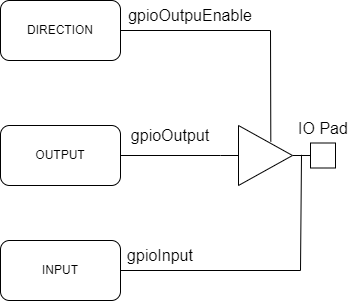
\includegraphics[width=0.4\textwidth]{images/ppl.png}
    \caption{Push Pull Mode}
  \end{figure}

\subsection{Open Drain Mode}
In this mode, each bit of gpioOutput is driven low when the corresponding OUTPUT register bit is low and corresponding DIRECTION register bit is high. 
This allows for multiple devices to pull the line low without conflicting high/low states on the output pin.

\begin{figure}[h]
    \centering
    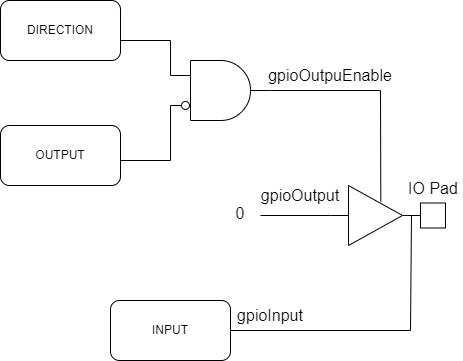
\includegraphics[width=0.4\textwidth]{images/od.drawio.png}
    \caption{Open Drain Mode}
  \end{figure}
\section{Virtual Ports}

\subsection{Introduction}
Virtual ports in the GPIO module allow for the abstraction of physical pins, enabling flexible control without altering the underlying hardware behavior. A virtual port can be mapped to a physical pin, and its behavior will correspond to the mode (input or output) of the pin it is mapped to.

This section details how virtual ports should behave when mapped to physical pins, how data flows between them, and how enable signals are managed.

\subsection{Physical Pin Configured as Output}
When the physical pin is configured as an output, the virtual port should mirror this configuration.

\begin{itemize}[noitemsep]
    \item \textbf{Data Flow}: The virtual port writes data to the corresponding physical pin.
    \begin{itemize}[noitemsep]
        \item Writing to the virtual port sets the output value of the physical pin.
        \item The virtual port is implicitly in output mode.
    \end{itemize}
    \item \textbf{Enable Behavior}: Writing to the virtual port acts as if writing directly to the physical pin.
    \begin{itemize}[noitemsep]
        \item Virtual port output is enabled when the physical pin output is enabled.
    \end{itemize}
\end{itemize}

\textbf{Example}:
\begin{itemize}[noitemsep]
    \item Physical pin $p$ is set as output.
    \item Virtual port $v$ is mapped to pin $p$.
    \item Writing a $1$ to virtual port $v$ sets the output of pin $p$ to $1$.
\end{itemize}

\subsection{Physical Pin Configured as Input}
When the physical pin is configured as an input, the virtual port should reflect the data from the physical pin.

\begin{itemize}[noitemsep]
    \item \textbf{Data Flow}: The virtual port reads the value of the physical pin.
    \begin{itemize}[noitemsep]
        \item Any read from the virtual port reflects the current value of the physical pin.
        \item The virtual port is implicitly in input mode.
    \end{itemize}
    \item \textbf{Enable Behavior}: Reading from the virtual port behaves as if reading directly from the physical pin.
    \begin{itemize}[noitemsep]
        \item Virtual port input is enabled when the physical pin input is enabled.
    \end{itemize}
\end{itemize}

\textbf{Example}:
\begin{itemize}[noitemsep]
    \item Physical pin $p$ is set as input.
    \item Virtual port $v$ is mapped to pin $p$.
    \item Reading from virtual port $v$ returns the current value of physical pin $p$ (either $0$ or $1$).
\end{itemize}

\subsection{Physical Pin Reconfiguration (Dynamic Behavior)}
If the direction of the physical pin changes dynamically during runtime, the virtual port should reflect this change.

\begin{itemize}[noitemsep]
    \item When a physical pin changes from \textbf{input to output}, the virtual port should switch from \textbf{read-only} to \textbf{write-enabled}.
    \item When a physical pin changes from \textbf{output to input}, the virtual port should switch from \textbf{write-enabled} to \textbf{read-only}.
    \item The virtual port should respect any changes to the physical pin's enable signal (e.g., when a pin is disabled or tri-stated).
\end{itemize}

\subsection{Summary of Correspondence}
The following table summarizes the behavior of virtual ports when mapped to physical pins.
\begin{table}[ht]
    \centering
    \resizebox{\textwidth}{!}{%
    \begin{tabular}{|c|c|c|c|}
        \hline
        \textbf{Physical Pin Mode} & \textbf{Virtual Port Behavior} & \textbf{Direction} & \textbf{Enable Behavior} \\ \hline
        \textbf{Output}            & Writes to virtual port propagate to physical pin & Implicit Output & Enabled if physical pin output is enabled \\ \hline
        \textbf{Input}             & Reads from virtual port reflect the physical pin value & Implicit Input  & Enabled if physical pin input is enabled  \\ \hline
    \end{tabular}%
    }
    \caption{Virtual Port Behavior Correspondence with Physical Pins}
\end{table}

\subsection{Additional Considerations}

\begin{itemize}[noitemsep]
    \item \textbf{Virtual-to-Physical Map}: Ensure that the \texttt{virtualToPhysicalMap} correctly identifies which physical pin a virtual port is mapped to and maintains this mapping throughout the operation.
    \item \textbf{Enable Flag}: The virtual port enable flag should be checked to ensure that virtual ports are supported. If not enabled, virtual ports should not interact with physical pins.
\end{itemize}

By maintaining consistent mapping and handling between virtual and physical ports, you ensure that virtual ports act as an abstraction layer, extending GPIO functionality without altering the behavior of the physical pins.

\section{Theory of Operations}

\subsection{Introduction}
The \textbf{DynamicFifo} is a highly parameterized FIFO and FIFO controller. It
is configurable as a full self-contained FIFO with internal memory being
constructed from flip-flops, or a FIFO controller that uses an external SRAM
for memory.

\begin{figure}[h]
  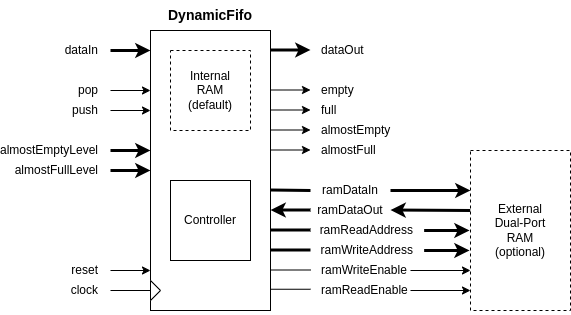
\includegraphics[width=0.80\textwidth]{images/block-diagram.png}
  \caption{Block Diagram}\label{fig:block-diagram}
\end{figure}

It features the following status flags which are described in
Table~\ref{table:ports}.

\begin{itemize}[noitemsep]
  \item{empty}
  \item{full}
  \item{almostEmpty}
  \item{almostFull}
\end{itemize}

When \textit{push} is asserted, the data on the \textit{dataIn} port is enqued
on the next rising edge of \textit{clock}. When \textit{pop} is asserted, the
top of the FIFO is dequed and immediately available on the \textit{dataOut}
port. Pop and Push operations can be simulataneous.

There are two error conditions which produce the following effects:
\begin{itemize}
  \item{When \textit{pop} is asserted and the FIFO is empty (\textit{empty} is
        active), \textit{dataOut} will contain the last valid data held in
        the FIFO.}
  \item{When \textit{push} is asserted and the FIFO is full (\textit{full} is
        active), \textit{dataIn} will be ignored and not enqued.}
\end{itemize}

The \textit{almostEmpty} and \textit{almostFull} flags allow for additional
feedback to the system that is useful for optimizing data flow control. The
levels of these flags can be programmed dynamically through the
\textit{almostEmptyLevel} and \textit{almostFullLevel} ports.

\newpage
\subsection{Interface Timing}

DynamicFifo has a simple, synchronous interface. The timing diagram shown below
in Figure~\ref{fig:timing} represents an instantiation with the following
parameters.

\begin{lstlisting}[language=Scala]
val myFifo = new DynamicFifo(
  externalRAM = true, 
  dataWidth = 16, 
  fifoDepth = 5) 
\end{lstlisting}

\begin{figure}[h]
  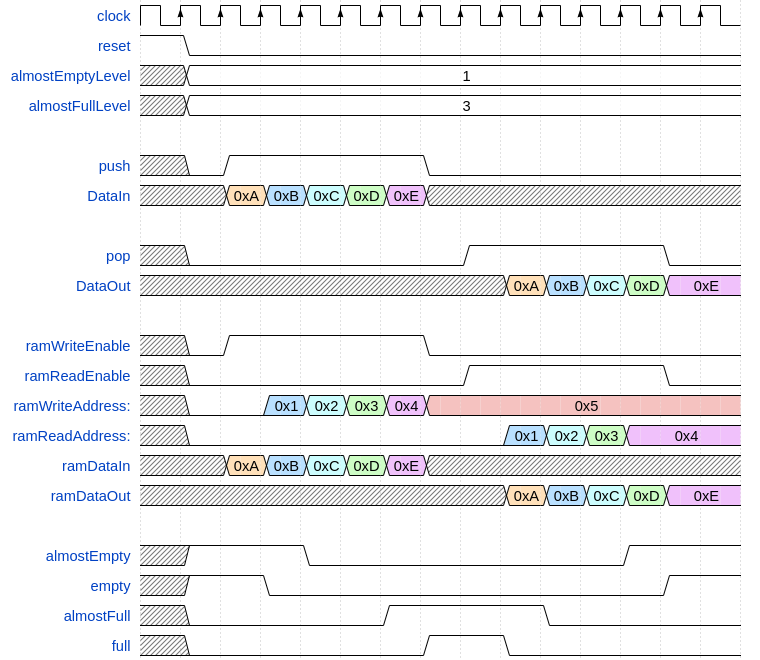
\includegraphics[width=\textwidth]{images/timing.png}
  \caption{Timing Diagram}\label{fig:timing}
\end{figure}

The \textit{almostEmptyLevel} port is driven by external logic to a static value
of 1 after reset and the \textit{almostFull} port is driven to 3.

Beginning in the third clock cycle, 5 words of data are pushed into the
FIFO.\ The status flags show the FIFO going from empty to full.

The FIFO is then fully emptied when the \textit{pop} port is help high for
5 clock cycles. The status flags show the FIFO going from full to empty again.
\section{Simulation}

\subsection{Tests}
The test bench generates a number (default is 50) configurations of the
DynamicFifo that are highly randomized. There are two flavors of tests:

\begin{itemize}
  \item {Directed tests that fill the FIFO with random data and then read back
        the results to verify that the read data matches the writted data.}
  \item {Lengthy random tests that are used to check odd combinations of
        configurations and to compile code coverage data.}
\end{itemize}

\subsection{Code coverage}
All inputs and outputs are checked to insure each toggle at least once. An error
will be thrown in case any port fails to toggle.

The only exception are the \emph{almostEmptyLevel} and \emph{almostFullLevel}
which are intended to be static during each simulation. These signals are
excluded from coverage checks.

\subsection{Running simulation}

Simulations can be run directly from the command prompt as follows:

\begin{verbatim}
  $ sbt "test"
\end{verbatim}

or from make as follows:

\texttt{\$ make test}
% chktex-file 44
\section{Synthesis}

\subsection{Area}

The DynamicFifo has been tested in a number of configurations and the following
results should be representative of what a user should see in their own
technology.

\renewcommand*{\arraystretch}{1.4}
\begin{longtable}[H]{
    | p{0.20\textwidth}
    | p{0.15\textwidth}
    | p{0.15\textwidth}
    | p{0.15\textwidth}
    | p{0.15\textwidth} |
  }
  \hline
  \textbf{Config Name}   &
  \textbf{externalRAM}   &
  \textbf{dataWidth}     &
  \textbf{fifoDepth}     &
  \textbf{Gates}           \\ \hline \hline

  small\_false\_8\_8     &
  false                  &
  8                      &
  8                      &
  769                      \\ \hline

  medium\_false\_32\_64  &
  false                  &
  32                     &
  64                     &
  19,283                   \\ \hline

  large\_false\_64\_256  &
  false                  &
  64                     &
  256                    &
  152,808                  \\ \hline

  small\_true\_64\_256   &
  true                   &
  64                     &
  256                    &
  355                      \\ \hline

  medium\_true\_128\_128 &
  true                   &
  128                    &
  128                    &
  477                      \\ \hline

  large\_true\_256\_2048 &
  true                   &
  256                    &
  2048                   &
  502                      \\ \hline
  \caption{Synthesis results}\label{table:area}
\end{longtable}

\subsection{SDC File}
An \texttt{.sdc} file is generated to provide synthesis and static timing
analysis tools guidance for synthesis.

The \texttt{DynamicFifo.sdc} file is emitted and found in the
\texttt{./syn} directory.

\subsection{Timing}

The following timing was extracted using the generated~.sdc files using the
Nangate 45nm free library.

\renewcommand*{\arraystretch}{1.4}
\begin{longtable}[H]{
    | p{0.20\textwidth}
    | p{0.08\textwidth}
    | p{0.12\textwidth}
    | p{0.13\textwidth}
    | p{0.15\textwidth}
    | p{0.15\textwidth} |
  }
  \hline
  \textbf{Config Name}   &
  \textbf{Period}        &
  \textbf{Duty Cycle}    &
  \textbf{Input Delay}   &
  \textbf{Output Delay}  &
  \textbf{Slack}           \\ \hline \hline

  small\_false\_8\_8     &
  5ns                    &
  50\%                   &
  20\%                   &
  20\%                   &
  2.93 (MET)               \\ \hline

  medium\_false\_32\_64  &
  5ns                    &
  50\%                   &
  20\%                   &
  20\%                   &
  2.69 (MET)               \\ \hline

  large\_false\_64\_256  &
  5ns                    &
  50\%                   &
  20\%                   &
  20\%                   &
  2.80 (MET)               \\ \hline

  small\_true\_64\_256   &
  5ns                    &
  50\%                   &
  20\%                   &
  20\%                   &
  2.80 (MET)               \\ \hline

  medium\_true\_128\_128 &
  5ns                    &
  50\%                   &
  20\%                   &
  20\%                   &
  2.70 (MET)               \\ \hline

  large\_true\_256\_2048 &
  5ns                    &
  50\%                   &
  20\%                   &
  20\%                   &
  2.77 (MET)               \\ \hline
  \caption{Static Timing Analysis results}\label{table:timing}
\end{longtable}

\subsection{Multicycle Paths}
None.


\end{document}
